\documentclass{article}

\usepackage{tikz}
\usepackage[inner=0.5cm,outer=0.5cm]{geometry}

\begin{document}
\subsection*{12 faces, mmm}
 \bigskip

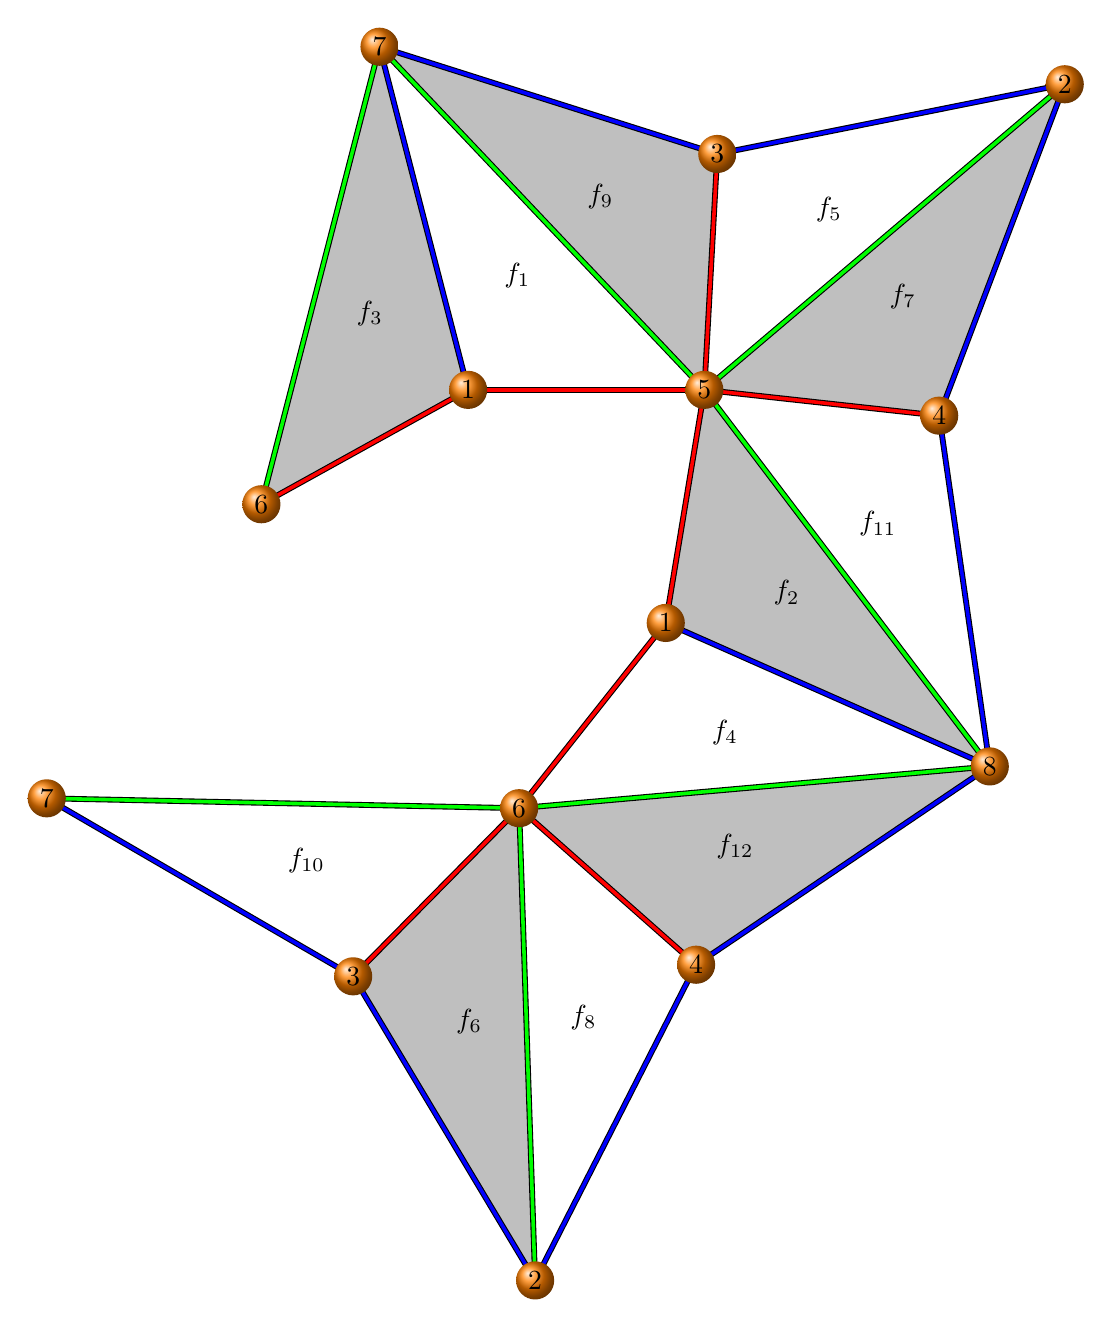
\begin{tikzpicture}[scale=3/2]
\coordinate (V1_1) at (0, 0);
\coordinate (V1_2) at (1.673183441162109, -1.973117061116588);
\coordinate (V2_1) at (5.05078125, 2.587031844536985);
\coordinate (V2_2) at (0.5672462582588191, -7.53908759171338);
\coordinate (V3_1) at (2.109375, 1.997007037888199);
\coordinate (V3_2) at (-0.973055306822062, -4.964700074533926);
\coordinate (V4_1) at (3.988037109375, -0.2184226447690221);
\coordinate (V4_2) at (1.930021047592163, -4.866477467965911);
\coordinate (V5_1) at (2, 0);
\coordinate (V6_1) at (-1.75, -0.9682458365518543);
\coordinate (V6_2) at (0.4319877624511719, -3.541375103388106);
\coordinate (V7_1) at (-0.75, 2.904737509655563);
\coordinate (V7_2) at (-3.567139173857867, -3.457806285713838);
\coordinate (V8_1) at (4.41632080078125, -3.187694117651796);


\fill[white] (V1_1) -- (V5_1) -- (V7_1) -- cycle;
\node (F1) at (0.4166666666666666, 0.9682458365518543) {$f_{1}$};
\fill[lightgray] (V1_2) -- (V5_1) -- (V8_1) -- cycle;
\node (F2) at (2.69650141398112, -1.720270392922794) {$f_{2}$};
\fill[lightgray] (V1_1) -- (V6_1) -- (V7_1) -- cycle;
\node (F3) at (-0.8333333333333333, 0.6454972243679029) {$f_{3}$};
\fill[white] (V1_2) -- (V6_2) -- (V8_1) -- cycle;
\node (F4) at (2.17383066813151, -2.90072876071883) {$f_{4}$};
\fill[white] (V2_1) -- (V3_1) -- (V5_1) -- cycle;
\node (F5) at (3.053385416666667, 1.528012960808395) {$f_{5}$};
\fill[lightgray] (V2_2) -- (V3_2) -- (V6_2) -- cycle;
\node (F6) at (0.008726237962643008, -5.34838758987847) {$f_{6}$};
\fill[lightgray] (V2_1) -- (V4_1) -- (V5_1) -- cycle;
\node (F7) at (3.679606119791667, 0.7895363999226543) {$f_{7}$};
\fill[white] (V2_2) -- (V4_2) -- (V6_2) -- cycle;
\node (F8) at (0.976418356100718, -5.315646721022465) {$f_{8}$};
\fill[lightgray] (V3_1) -- (V5_1) -- (V7_1) -- cycle;
\node (F9) at (1.119791666666667, 1.633914849181254) {$f_{9}$};
\fill[white] (V3_2) -- (V6_2) -- (V7_2) -- cycle;
\node (F10) at (-1.369402239409586, -3.987960487878623) {$f_{10}$};
\fill[white] (V4_1) -- (V5_1) -- (V8_1) -- cycle;
\node (F11) at (3.468119303385417, -1.135372254140273) {$f_{11}$};
\fill[lightgray] (V4_2) -- (V6_2) -- (V8_1) -- cycle;
\node (F12) at (2.259443203608195, -3.865182229668604) {$f_{12}$};


\tikzset{EdgeStyle/.style = {thin, double distance=1.3pt} }

\draw[ EdgeStyle, double=red] (V5_1) -- (V1_1);
\draw[ EdgeStyle, double=red] (V1_2) -- (V5_1);
\draw[ EdgeStyle, double=red] (V1_1) -- (V6_1);
\draw[ EdgeStyle, double=red] (V6_2) -- (V1_2);
\draw[ EdgeStyle, double=blue] (V1_1) -- (V7_1);
\draw[ EdgeStyle, double=blue] (V8_1) -- (V1_2);
\draw[ EdgeStyle, double=blue] (V3_1) -- (V2_1);
\draw[ EdgeStyle, double=blue] (V2_2) -- (V3_2);
\draw[ EdgeStyle, double=blue] (V2_1) -- (V4_1);
\draw[ EdgeStyle, double=blue] (V4_2) -- (V2_2);
\draw[ EdgeStyle, double=green] (V2_1) -- (V5_1);
\draw[ EdgeStyle, double=green] (V2_2) -- (V6_2);
\draw[ EdgeStyle, double=red] (V3_1) -- (V5_1);
\draw[ EdgeStyle, double=red] (V3_2) -- (V6_2);
\draw[ EdgeStyle, double=blue] (V7_1) -- (V3_1);
\draw[ EdgeStyle, double=blue] (V3_2) -- (V7_2);
\draw[ EdgeStyle, double=red] (V4_1) -- (V5_1);
\draw[ EdgeStyle, double=red] (V4_2) -- (V6_2);
\draw[ EdgeStyle, double=blue] (V4_1) -- (V8_1);
\draw[ EdgeStyle, double=blue] (V8_1) -- (V4_2);
\draw[ EdgeStyle, double=green] (V7_1) -- (V5_1);
\draw[ EdgeStyle, double=green] (V8_1) -- (V5_1);
\draw[ EdgeStyle, double=green] (V6_1) -- (V7_1);
\draw[ EdgeStyle, double=green] (V7_2) -- (V6_2);
\draw[ EdgeStyle, double=green] (V8_1) -- (V6_2);



\tikzset{VertexStyle/.style = {
 shape = circle,
 ball color = orange,
 text = black,
 inner sep = 2pt,
 outer sep = 0pt,
 minimum size = 10pt} }

\node[VertexStyle] at (V1_1) {1};
\node[VertexStyle] at (V1_2) {1};
\node[VertexStyle] at (V2_1) {2};
\node[VertexStyle] at (V2_2) {2};
\node[VertexStyle] at (V3_1) {3};
\node[VertexStyle] at (V3_2) {3};
\node[VertexStyle] at (V4_1) {4};
\node[VertexStyle] at (V4_2) {4};
\node[VertexStyle] at (V5_1) {5};
\node[VertexStyle] at (V6_1) {6};
\node[VertexStyle] at (V6_2) {6};
\node[VertexStyle] at (V7_1) {7};
\node[VertexStyle] at (V7_2) {7};
\node[VertexStyle] at (V8_1) {8};

\end{tikzpicture}

\end{document} 
